\chapter{Event sufficient conditions}\label{parEventSufficientConditions}%
\addcontentsline{itc}{chapter}{\protect\numberline{\thechapter}Event sufficient conditions}

In \S~\ref{parpro0699} we saw that the maximal correlation coefficient $\{\mathcal{F}:\mathcal{G}\}$
controls the difference between~$\Pr[A \cap B]$ and~$\Pr[A]\Pr[B]$
for~$A$ and~$B$ two events resp.\ $\mathcal{F}$- and $\mathcal{G}$-measurable.
A natural question is whether the converse is true,
i.e.\ whether saying that $\Pr[A\cap B]$ is always close in some sense to~$\Pr[A]\Pr[B]$
implies a control on~$\{\mathcal{F}:\mathcal{G}\}$.
We saw in \S~\ref{parAlphaMixing} that $\alpha$-mixing does not fit,
but maybe stronger conditions of the same type would work.

In \S~\ref{parWeakEventSufficientCondition}
I will present a simple such condition (Theorem~\ref{thm0367a}).
This condition demands $|\Pr[A\cap B]-\Pr[A]\Pr[B]|$ to be bounded uniformly
by~$\zeta(\Pr[A])\*\,\theta(\Pr[B])$ for functions $\zeta,\theta \colon [0,1] \to \RR_+$
sufficiently well behaved.
This result, whose proof is rather simple, is apparently new.

Proposition~\ref{pro0699}, however, suggests that the natural condition on events
would be a uniform control on
$\big|\Pr[A\cap B]-\Pr[A]\Pr[B]\big| \mathbin{\big/} \sqrt{\Pr[\C{A}]\Pr[A]}\sqrt{\Pr[\C{B}]\Pr[B]}$,
which is out of the scope of Theorem~\ref{thm0367a}.
Bradley~\cite{Bradley83} proved in 1983 that
that condition was indeed sufficient to get $\rho$-mixing.
His result was improved in the next few years
(see for instance the bound of~\cite{Bulinskii84}),
but the optimal bound was remaining unknown,
though its value was being conjectured.
In \S~\ref{parStrongEventSufficientCondition}, I shall prove this optimal bound.
My method, different from the techniques of~\cite{Bradley83, Bulinskii84},
relies on the analysis of the spectral properties of an operator linked to a law
which I call the ``Chogosov law'', whose study is proceeded to in \S~\ref{parTheChogosovProcess}.


\section{Weak event sufficient condition}\label{parWeakEventSufficientCondition}

To state our next result we need some functional analysis reminders first:
\begin{Def}
On the space $\mathcal{C}^{\infty}_0(0,1)$ of compactly supported fuctions of~$\mathcal{C}^{\infty}(0,1)$,
one defines the scalar product
\[ \langle\phi,\psi\rangle_{H^1_0} = \int_0^1 \phi'(x)\psi'(x) \,\dx{x} .\]
$\mathcal{C}^{\infty}_0(0,1)$ endowed with~$\langle\Bcdot,\Bcdot\rangle_{H^1_0}$ is a pre-Hilbert space;
its completion is denoted by~$H^1_0(0,1)$.
\end{Def}
%
Recall that elements of~$H^1_0(0,1)$ may be seen as ordinary functions:
\begin{Lem}[Sobolev, {\cite[Theorem~4.12]{Sobolev}}]\label{lem9060}
Any element $f \in H^1_0(0,1)$ can be identified with a unique function
$\bar{f} \in \mathcal{C}^0_0[0,1]$, the space of continuous functions on~$[0,1]$
with $\bar{f}(0), \bar{f}(1) = 0$.
Conversely, a function~$\bar{f} \in \mathcal{C}^0_0[0,1]$ corresponds to
an element of~$H^1_0(0,1)$ if and only if
\[\label{for9029}
\sup_{g\in\mathcal{C}^{\infty}_0(0,1)}
\frac{\big|\int_0^1 f(x)g''(x)\dx{x}\big|}{\sqrt{\int_0^1 g'(x)^2\dx{x}}} \]
is finite, and then there is a unique $f\in H^1_0(0,1)$ associated to~$\bar{f}$,
whose norm is~(\ref{for9029}).
\end{Lem}
%
In accordance with Lemma~\ref{lem9060}, we will identify functions of~$\mathcal{C}^0_0[0,1]$
with elements of~$H^1_0(0,1)$ whenever it is possible. If $f\in\mathcal{C}^0_0[0,1]$
does not correspond to an element of~$H^1_0(0,1)$, then we will set $\|f\|_{H^1_0} = +\infty$.

Now we can state the
%
\begin{Thm}[Weak event sufficient condition]\label{thm0367a}
Let~$\mathcal{F}$ and~$\mathcal{G}$ be two $\sigma$-algebras
such that, for all~$A\in\mathcal{F}$ and~$B\in\mathcal{G}$
with respective probabilities~$p$ and~$q$,
\[\label{for0256} \Pr[A\cap B]-pq \leq \zeta(p)\theta(q) \footnotemark\]
\footnotetext{Note that there is no need to put absolute values
in the left-hand side of (\ref{for0256}).}%
for some $\zeta, \theta \in \mathcal{C}^0_0[0,1]$.
Then:
\[\label{for0458} \{\mathcal{F}:\mathcal{G}\} \leq \|\zeta\|_{H^1_0} \|\theta\|_{H^1_0} .\]
\end{Thm}

\begin{proof}
We begin with the following formula for covariance:
\begin{Lem}\label{lem8312}
For~$f$ and~$g$ two real $L^2$ functions,
\[\label{for0257}
\Cov(f,g) = \int_{\RR\times\RR}
\big( \Pr[f\leq x\text{ and }g\leq y] - \Pr[f\leq x] \Pr[g\leq y]\big) \,\dx{x}\dx{y} .\]
\end{Lem}
%
\begingroup\def\proofname{Proof of Lemma~\ref{lem8312}}
\begin{proof}
Suppose in a first time that $f$ and~$g$ are nonnegative.
A classical Fubini argument (see \cite[Problem~21.6]{Billingsley*})
shows that
\[ \EE[f] = \int_{\RR_+} \Pr[f>x] \,\dx{x} ,\]
with a similar formula for~$g$. By the same method,
\[ \EE[fg] = \int_{\RR_+\times\RR_+} \Pr[f>x \text{ and } g>y] \,\dx{x}\dx{y} ,\]
so that, using the computational formula $\Cov(f,g) = \EE[fg] - \EE[f]\EE[g]$,
\[ \Cov(f,g) = \int_{\RR_+\times\RR_+}
\big( \Pr[f>x\text{ and }g>y] - \Pr[f>x] \Pr[g>y] \big) \,\dx{x}\dx{y}.\]
Observing that the integrand is also
$( \Pr[f\leq x\text{ and }g\leq y] - \Pr[f\leq x] \Pr[g\leq y] )$
and that it is zero for~$(x,y) \notin \RR_+ \times \RR_+$,
we get~(\ref{for0257}) in the nonnegative case.
By translation invariance, the formula remains true for all~$f,g$ bounded below,
and then by approximation for all~$f,g \in L^2$.
\end{proof}\endgroup

Now, let~$f$ and~$g$ be $L^2$ variables resp.\ $\mathcal{F}$- and $\mathcal{G}$-mesurable,
and denote by~$F$ and~$G$ the respective distribution functions of~$f$ and~$g$.
Up to a slight perturbation, $F$ and~$G$
may be supposed to be diffeomorphisms from~$\RR$ onto~$(0,1)$;
denote by~$\alpha$ and~$\beta$ their respective inverse maps.
Then a change of variables in (\ref{for0257}) yields:
\[\label{for0268} \Cov(f,g) = \int_{(0,1)^2}
\Big( \Pr\big[f\leq \alpha(p)\text{ and }g\leq \beta(q)\big] - pq \Big)
\alpha'(p)\beta'(q) \,\dx{p}\dx{q} ,\]
so by assumption (\ref{for0256}):
\[\label{for9181}
\Cov(f,g) \leq \Big(\int_0^1\zeta(p)\alpha'(p) \,\dx{p}\Big) \times
\Big(\int_0^1\theta(q)\beta'(q) \,\dx{q}\Big) .\]
Then our theorem becomes equivalent to the claim stated and proved just below.
\end{proof}
%
\begin{Clm}\label{clm6860}
If $f$ is a random variable whose repartition function~$F$ is a diffeomorphism
of inverse~$\alpha$, then for~$\zeta \in \mathcal{C}^0_0[0,1]$:
\[ \Big| \int_0^1 \zeta(p)\alpha'(p)\dx{p} \Big| \leq \|\zeta\|_{H^1_0} \ecty(f) .\]
\end{Clm}

\begin{proof}
First note that, replacing $g$ by~$f$ in~(\ref{for0268}),
one has:
\[ \Var(f) = \int_{(0,1)^2} \big[ p(1-q) \wedge q(1-p) \big] \alpha'(p)\alpha'(q) \,\dx{p}\dx{q} .\]
In fact, one can define a scalar product%
\footnote{The positivity of~$\langle\Bcdot,\Bcdot\rangle_V$ follows from the identity
$\langle\phi,\phi\rangle_V = \int_{p<q} \big( \int_p^q \phi(r) \,\dx{r} \big)^2 \,\dx{p}\dx{q}$.}
$\langle\Bcdot,\Bcdot\rangle_V$ on~$\mathcal{C}^0(0,1)$ by setting
\[ \label{for0312}
\langle\phi,\psi\rangle_{V} = \int_{(0,1)^2} \big[ p(1-q) \wedge q(1-p) \big] \phi(p)\psi(q) \,\dx{p}\dx{q} ,\]
so that if $\alpha$ is the inverse distribution fuction
of a variable $f$, $\Var(f) = \|\alpha'\|_V^2$.

So, we are considering three scalar products on some subspaces of~$\mathcal{C}^0(0,1)$:
the ordinary $L^2$ product, which we denote by~$\langle\Bcdot,\Bcdot\rangle_{L^2}$,
the $H^1_0(0,1)$ product $\langle\Bcdot,\Bcdot\rangle_{H^1_0}$
and the variance product $\langle\Bcdot,\Bcdot\rangle_{V}$.
Our goal is to show that for all~$\phi \in H^1_0(0,1), \psi \in \mathcal{C}^0(0,1)$,
\[\label{for0032}
\big| \langle \phi,\psi \rangle_{L^2} \big| \leq \|\phi\|_{H^1_0} \|\psi\|_{V} .\]

By approximation we can suppose that $\phi\in\mathcal{C}^{\infty}_0(0,1)$.
A direct computation shows that
\[ \langle\phi,\psi\rangle_V = \langle L\phi,\psi\rangle_{L^2} ,\]
where the operator $L \colon \mathcal{C}^{\infty}_0(0,1) \to \mathcal{C}^2(0,1)$ is defined by:
\[\label{for0269} \big(L\phi\big)(x) = x\int_0^x (1-y)\phi(y) \,\dx{y} + (1-x)\int_x^1 y\phi(y) \,\dx{y} .\]
%
But we can make $L$ appear thanks to the following formula:
for~$\phi \in \mathcal{C}^2_0(0,1)$,
\[ \phi = L(-\phi'') ,\]
as one checks by integrating by parts twice.
So,
\[ \big|\langle\phi,\psi\rangle_{L^2}\big| = \big|\langle L(-\phi''),\psi\rangle_{L^2}\big|
= \big|\langle-\phi'',\psi\rangle_V\big| \footrel{\text{CS}}{\leq} \| \phi'' \|_V \| \psi \|_V ,\]
where
\[ \|\phi''\|_V^2 = \langle\phi'',\phi''\rangle_V = \langle L\phi'',\phi''\rangle_{L^2} = -\langle\phi,\phi''\rangle_{L^2}
\footrel{\text{IP}}{=} \|\phi'\|_{L^2}^2 = \|\phi\|_{H^1_0}^2 ,\]
whence~(\ref{for0032}).
\end{proof}


\section{Strong event sufficient condition}\label{parStrongEventSufficientCondition}

\subsection{The strong event sufficient condition}\label{parTheStrongEventSufficientCondition}

A natural choice for functions~$\zeta$ and~$\theta$ in Theorem~\ref{thm0367a}
would be $\zeta(p) = \theta(p) = \epsilon^{1/2} \* \sqrt{p(1-p)}$,
since that would give a converse to Formula~(\ref{for3346}) of Proposition~\ref{pro0699}.
Unfortunately $\| \sqrt{p(1-p)} \|_{H^1_0} = +\infty$,
so Theorem~\ref{thm0367a} does not work in this case.
There is however a specific result then:

\begin{Thm}[Strong event sufficient condition]\label{thm0367b}
Let~$\mathcal{F}$ and~$\mathcal{G}$ be two $\sigma$-algebras
such that, for all~$A$ and~$B$ resp.\ in~$\mathcal{F}$ and~$\mathcal{G}$
with respective probabilities~$p$ and~$q$,
\[\label{for0256b} \Pr[A\cap B]-pq \leq \epsilon \sqrt{p(1-p)q(1-q)} \]
for some $\epsilon\in[0,1]$.
Then
\[\label{for7753} \{\mathcal{F}:\mathcal{G}\} \leq \Lambda(\epsilon) ,\]
where $\Lambda \colon [0,1] \to \RR_+$ is defined by
\[ \Lambda(\epsilon) \coloneqq \begin{cases} \epsilon (1+|\ln\epsilon|) & \text{if $\epsilon>0$,} \\
0 & \text{if $\epsilon=0$.} \end{cases}\]
\end{Thm}

\begin{Rmk}
The function~$\Lambda$ is increasing on~$[0,1]$ and satisfies
$\Lambda(0)=0$, $\Lambda(1)=1$, and $\Lambda(\epsilon)>\epsilon$
for all~$\epsilon\in(0,1)$.
Moreover it is continuous, in particular
$\Lambda(\epsilon) \searrow 0$ as $\epsilon \searrow 0$
(see Figure~\ref{fig-Lambda}).
\end{Rmk}
%
\begin{figure}
\centering
%
\begin{tikzpicture}[x=4cm, y=4cm, line cap=round, >=stealth]

\draw[->,thin] (0,0) node[anchor=north]{$0$} -- node[anchor=north]{$x$} (1,0) node[anchor=north]{$1$} ;
\draw[->,thin] (0,0) node[anchor=east ]{$0$} -- node[anchor=east ]{$y$} (0,1) node[anchor=east ]{$1$} ;
\draw[thin,dotted] (0,1) -- (1,1) ;
\draw[thin,dotted] (1,0) -- (1,1) ;
\draw[thick] plot[smooth] file{Lambda.txt} ;
\path (.36788,.73576) +(-1pt,-1pt) -- node[above,sloped]{$y=\Lambda(x)$} +(1pt,1pt) ;
\draw[very thin] (0,0) -- node[midway,below,sloped]{$y=x$} (1,1) ;

\end{tikzpicture}
%
\caption{The function~$\Lambda$.}\label{fig-Lambda}
%
\end{figure}


\begin{Rmk}
I called Theorems~\ref{thm0367a} and~\ref{thm0367b}
resp.\ ``weak'' and ``strong'' event sufficient conditions;
yet that vocabulary is a bit misleading,
since the strong condition does not imply the weak one \emph{stricto sensu}:
with the hypotheses of Theorem~\ref{thm0367a} indeed,
Theorem~\ref{thm0367b} only implies that
\[\label{fo1611} \{\mathcal{F}:\mathcal{G}\} \leq \Lambda\big(\|\zeta\|_{H^1_0}\|\theta\|_{H^1_0}\big) .\]
But the right-hand side of~(\ref{fo1611}) tends to~$0$
as soon the right-hand side of~(\ref{for0458}) does,
so it is relevant to say that Theorem~\ref{thm0367b} is `qualitatively stronger'
than Theorem~\ref{thm0367a}.
\end{Rmk}

\begin{Rmk}
With the same informal vocabulary,
Theorem~\ref{thm0367b} is a `qualitative converse' of Proposition~\ref{pro0699}:
maximal decorrelation is `qualitatively equivalent' to decorrelation of events
as defined by Formula~(\ref{for3346}).
\end{Rmk}

\begin{Rmk}
One can prove that the bound $\Lambda(\epsilon)$
in~(\ref{for7753}) is the best possible:
see \S~\ref{parOptimalityOfTheStrongEventSufficientCondition}.
\end{Rmk}

\begin{proof}
The core principle of the proof is the same as for Theorem~\ref{thm0367a},
except that we first perform a tricky refinement of the hypothesis:
observing that, for~$A$ and~$B$ with respective probabilities~$p$ and~$q$,
one trivially has $\Pr[A\cap B] \leq p\wedge q$,
the bound~(\ref{for0256b}) can be strengthened into:
\[\label{for0256c} \Pr[A\cap B] \leq \big( pq + \epsilon\sqrt{p(1-p)q(1-q)} \big) \wedge p\wedge q .\]
The right-hand side of~(\ref{for0256c}) will be denoted by~$Z_{\epsilon}(p,q)$.

Now, like in the proof of Theorem~\ref{thm0367a},
if (\ref{for0256b}) is satisfied, for $f$ and~$g$ two $L^2$ real variables
resp.\ $\mathcal{F}$- and $\mathcal{G}$-measurable, having respective distribution functions~$F$ and~$G$
with respective inverses maps~$\alpha$ and~$\beta$:
\[\label{for0268b} \Cov(f,g) \leq \int_{(0,1)^2} \big(Z_{\epsilon}(p,q)-pq\big) \alpha'(p)\beta'(q)
\, \dx{p}\dx{q} .\]
Call~$\langle\alpha',\beta'\rangle_{Z_\epsilon}$ the right-hand side of~(\ref{for0268b}).

To bound $\langle\alpha',\beta'\rangle_{Z_\epsilon}$,
this time we are remaining on a random variable paradigm:
%
\begin{Def}\label{def5228}
The \emph{Chogosov law}%
\footnote{So called in honour of my dear friend M.~K.~Chogosov.}
is the (unique) probability measure $\mu$ on~$(0,1)^2$ such that
\[\label{for0229}
\forall (p,q) \in (0,1)^2 \qquad \mu\big[ (0,p) \times (0,q) \big] = Z_\epsilon(p,q) .\]
\end{Def}
%
It shall be proved in \S~\ref{parTheChogosovProcess} that the Chogosov law actually exists.
$\mu$ is invariant under switching $x_1$ and~$x_2$ as the function $Z(p,q)$ is,
and its marginals are uniform on~$(0,1)$ as $Z(p,1) \equiv p$.

The Chogosov law is linked to~$\langle\Bcdot,\Bcdot\rangle_{Z_{\epsilon}}$ by the operator defined next:
%
\begin{Def}
For $p\in(0,1)$, denote by $\mu_p$ the conditional law of~$x_2$ knowing that $x_1=p$ under~$\mu$:
$(\mu_p)_{p\in(0,1)}$ is the family of probability laws on~$(0,1)$ such that for all measurable $X\subset(0,1)^2$,
\[ \mu[X] = \int_0^1 \mu_p [\{q\colon (p,q)\in X\}] \,\dx{p} .\footnotemark\]
\footnotetext{\emph{Stricto sensu} the family of measures $(\mu_p)_{p\in(0,1)}$
is only defined up to a.s.\ equality; however, this family has a unique version such that
$p \mapsto \mu_p$ is continuous for the weak convergence of measures,
which is the one that we will consider in the sequel.}
\end{Def}
%
\begin{Def}
Let~$\mcal{L}$ be the operator on bounded functions on~$(0,1)$ defined by
\[ (\mcal{L}\beta)(p) \coloneqq \int_0^1 \beta(q) \,\dx{\mu_p}[q] ;\]
in other words, $\mcal{L}$ is the generator of the stationary Markow chain
$\ldots \to r_0 \to r_1 \to \ldots$ with uniform equilibrium measure on~$(0,1)$
such that the $(r_i,r_{i+1})$ have law~$\mu$.
\end{Def}
%
\noindent Then the very definition of~$\langle\Bcdot,\Bcdot\rangle_{Z_{\epsilon}}$ yields:
\[ \langle\alpha',\beta'\rangle_{Z_{\epsilon}} = \Cov(\alpha,\mathcal{L}\beta) ,\]
%
where by writing ``$\Cov(\alpha,\mathcal{L}\beta)$'' I consider
functions~$\alpha$ and~$\mathcal{L}\beta$ as real random variables
on the probability space $(0,1)$ endowed with the uniform measure.

By the Cauchy--Schwarz inequality,
it is then enough to prove that $\Var(\mathcal{L}\beta) \leq \Lambda(\epsilon)\Var(\beta)$,
i.e.\ that the operator norm of~$\mathcal{L}$ on~$\ldb(0,1)$ is bounded above by~$\Lambda(\epsilon)$.
That work is achieved by Lemma~\ref{lem7792} in next subsection.
\end{proof}


\subsection{The Chogosov law}\label{parTheChogosovProcess}

This subsection deals with the ``Chogosov law'',
which we introduced in the proof of Theorem~\ref{thm0367b}.

\begin{NOTA}
Throughout this subsection we suppose $\epsilon\in(0,1)$ fixed
and we write~$\Lambda$ for~$\Lambda(\epsilon)$, resp.~$Z$ for~$Z_{\epsilon}$.
The drawings will be made for $\epsilon=1/2$.
\end{NOTA}

Recall Definition~\ref{def5228} of the Chogosov law.
We first have to check that the Chogosov law actually exists:
%
\begin{Clm}\label{clm4375}
There exists a (unique) probability measure~$\mu$ on~$(0,1)^2$ such that
\[\label{for7083}
\forall p,q \in [0,1] \quad \mu\big[\big\{(x_1,x_2)\in(0,1)^2 \colon 
x_1\leq p \text{ and } x_2\leq q\big\}\big] = Z(p,q) ,\]
where we recall that
\[ Z(p,q) \coloneqq \big( pq + \epsilon\sqrt{p(1-p)q(1-q)} \big) \wedge p\wedge q .\]
\end{Clm}

\begin{proof}
(\ref{for7083}) means that the density of~$\mu$ on~$(0,1)^2$ is equal to the distribution
$\partial^2_{x_1x_2}Z$; the non-trivial point consists in proving that
that distribution is nonnegative.

\begin{NOTA}
From now on in this subsection elements of~$(0,1)^2$ will be automatically denoted by~$(p,q)$.
Moreover, we will denote $\bar{p} \coloneqq 1-p$ and $\tilde{p} \coloneqq p-1/2$,
resp.\ $\bar{q} \coloneqq 1-q$ and $\tilde{q} \coloneqq q-1/2$.
\end{NOTA}

The analytic formula defining $Z(p,q)$ depends on the zone of~$(0,1)^2$
in which $(p,q)$ lies (see Figure~\ref{fig-mu}):
\begin{itemize}
\item If $p\bar{q} \div q\bar{p} \leq \epsilon^2$, then $Z(p,q) = p$ and we will say that we are in zone~\onecirc;
\item If $\epsilon^2 \leq p\bar{q} \div q\bar{p} \leq \epsilon^{-2}$, then $Z(p,q) = pq + \sqrt{p\bar{p}q\bar{q}}$
and we will say that we are in zone~\twocirc;
\item If $\epsilon^{-2} \leq p\bar{q} \div q\bar{p}$, then $Z(p,q) = q$ and we will say that we are in zone~\threecirc.
\end{itemize}
%
\begin{figure}
\centering
%
%% Le dessin du fuseau "nu".
%
\begin{tikzpicture}[x=5.25cm, y=5.25cm, line cap=round, >=stealth]

%% Le carré contenant le fuseau.

\draw[->,thin] (0,0) node[anchor=north]{$0$} -- node[midway,anchor=north]{$p$} (1,0) node[anchor=north]{$1$};
\draw[->,thin] (0,0) node[anchor=east ]{$0$} -- node[midway,anchor=east ]{$q$} (0,1) node[anchor=east ]{$1$};
\draw[thin,dotted] (1,0) -- (1,1);
\draw[thin,dotted] (0,1) -- (1,1);

%% Dessin du fuseau.

\draw[thick] plot[smooth] file {fuseauD.txt};
\draw[thick] plot[smooth] file {fuseauU.txt};

%% Nom des zones.

\node at (.167,.833) {\onecirc};
\node at (.500,.500) {\twocirc};
\node at (.833,.167) {\threecirc};

%% Nom des lignes.

\coordinate (ligneD) at (0.25000, 0.07692) {};
\coordinate (ligneU) at (0.75000, 0.92308) {};
\path (ligneD) +(0,.125) node[inner sep=1pt] (nomD) {$\mfrak{D}$};
\path (ligneU) +(0,-.125) node[inner sep=1pt] (nomU) {$\mfrak{U}$};
\draw[<-] (ligneD) -- (nomD) ;
\draw[<-] (ligneU) -- (nomU) ;
\end{tikzpicture}
%
\hfill
%
%% Le nuage de points.
%
\begin{tikzpicture}[x=5.25cm, y=5.25cm, line cap=round, >=stealth]

%% Le carré contenant le fuseau.

\draw[->,thin] (0,0) node[anchor=north]{$0$} -- node[midway,anchor=north]{$p$} (1,0) node[anchor=north]{$1$};
\draw[->,thin] (0,0) node[anchor=east ]{$0$} -- node[midway,anchor=east ]{$q$} (0,1) node[anchor=east ]{$1$};
\draw[thin,dotted] (0,1) -- (1,1);
\draw[thin,dotted] (1,0) -- (1,1);

%%Les 2048 points.

\begin{scope}[ultra thin]
\input{mu-data-2048}
\end{scope}
\end{tikzpicture}
%
\caption{The Chogosov law~$\mu$. On the left
are drawn the different zones relative to the support of the measure;
on the right is a cloud of 2,048 independent points with law $\mu$.}%
\label{fig-mu}
%
\end{figure}

So the expression of~$\partial_pZ$ depends on the zone where one lies:
in~\onecirc\ it is ``$1$'', in~\twocirc\ it is
``$q-\epsilon\tilde{p}\sqrt{q\bar{q} \div p\bar{p}}$'',
and in~\threecirc\ it is ``$0$''. Anyway it is defined and finite evererywhere,
just having jumps at the borders between the zones, which borders we will denote
respectively $\mfrak{U}$ for the border between~\onecirc\ and~\twocirc,
and $\mfrak{D}$ for the border between~\twocirc\ and~\threecirc\ (see Figure~\ref{fig-mu}).
To prove that the distribution~$\partial^2_{pq}Z$ is nonnegative, we have to show
that $\partial_pZ$ is increasing in~$q$ at~$p$ fixed.
Let us check it:
%
\begin{itemize}
\item In~\onecirc\ and~\threecirc, $\partial_pZ$ is differentiable with
$\partial_q(\partial_pZ) = 0 \geq 0$;
%
\item In~\twocirc, $\partial_pZ$ is differentiable with
$\partial_q(\partial_pZ) = 1 + \epsilon \tilde{p}\tilde{q} \div \sqrt{p\bar{p}q\bar{q}}$.
Denoting by~$\rho(p,q)$ that expression, let us prove that
$\rho(p,q)$ is nonnegative (and even positive) in~\twocirc:
either $\tilde{p}$ and~$\tilde{q}$ have the same sign and then $\rho(p,q)$ is trivially $\geq 1$,
or $\tilde{p}$ and~$\tilde{q}$ have opposite signs.
In the latter case, say for instance that $(\tilde{p}\geq0\enskip\text{and}\enskip \tilde{q}\ \leq 0)$.
Then $p\geq1/2$ and $q\leq1/2$, so $|\tilde{p}|=p-1/2<p$
and $|\tilde{q}|=1/2-q<\bar{q}$, which implies that
\[ \epsilon \frac{|\tilde{p}\tilde{q}|}{\sqrt{p\bar{p}q\bar{q}}}
< \epsilon \sqrt{\frac{p\bar{q}}{q\bar{p}}} \stackrel{\twocirc}{\leq} \epsilon\sqrt{\epsilon^{-2}} = 1 ,\]
so that $\rho(p,q) > 0$.
%
\item On~$\mfrak{D}$, $\partial_pZ$ makes a jump. Denote by~$q^{\mfrak{D}}_p$ the unique
$q$ such that $(p,q)\in\mfrak{D}$. When~$q$ tends to~$q^{\mfrak{D}}_p$ by lower values,
$(p,q)$ is in \threecirc, so $\partial_pZ(p,q^{\mfrak{D}}_p-) = 0$,
while when~$q$ tends to~$q^{\mfrak{D}}_p$ by upper values,
$(p,q)$ is in \twocirc, so $\partial_pZ(p,q^{\mfrak{D}}_p+) =
q^{\mfrak{D}}_p-\epsilon\tilde{p}\sqrt{q^{\mfrak{D}}_p\bar{q}^{\mfrak{D}}_p \div p\bar{p}}$.
But on~$\mfrak{D}$, $q\bar{p} = \epsilon^2p\bar{q}$, so
\[ q^{\mfrak{D}}_p- \epsilon\tilde{p}\sqrt{\frac{q^{\mfrak{D}}_p\bar{q}^{\mfrak{D}}_p}{p\bar{p}}}
= q^{\mfrak{D}}_p - \epsilon\tilde{p}\sqrt{\frac{(q^{\mfrak{D}}_p)^2}{\epsilon^2p^2}}
= q^{\mfrak{D}}_p \bigg( 1 - \frac{\tilde{p}}{p} \bigg) = \frac{q^{\mfrak{D}}_p}{2p} > 0 ,\]
so that the jump of~$\partial_pZ(p,\Bcdot)$ at~$q^{\mfrak{D}}_p$
occurs in the increasing sense.
%
\item Similarly we find that on~$\mfrak{U}$, with obvious notation,
$\partial_pZ(p,q^{\mfrak{U}}_p+) - \partial_pZ(p,q^{\mfrak{U}}_p-) = \bar{q}^{\mfrak{U}}_p \div 2\bar{p} > 0$.
\end{itemize}
So we have proved that $\partial_pZ(p,q)$ is increasing in~$q$, which is what we wanted.
\end{proof}

\begin{Rmk}\label{rmk5379}
The measure~$\mu$ has a rather complicated structure:
it is supported by zone~\twocirc; it has density
$1+\epsilon\tilde{p}\tilde{q} \div \sqrt{p\bar{p}q\bar{q}}$ w.r.t.\ the Lebesgue measure
in the interior of that zone,
and on its boundaries it has a \emph{linear} density giving a mass $(q\div 2p)\,\dx{p}$
to the infinitesimal part of~$\mfrak{D}$ of abscissa~$p$,
resp.\ a mass $(\bar{q}\div 2\bar{p})\,\dx{p}$ to the infinitesimal part of~$\mfrak{U}$ of abscissa~$p$.
See Figure~\ref{fig-mu}.
\end{Rmk}

Now that its existence is ensured, we notice a crucial property of the operator~$\mcal{L}$:
%
\begin{Pro}\label{pro1288}
$\mcal{L}$ is self-adjoint on~$L^2(0,1)$.
\end{Pro}
%
\begin{Rmk}
As $\mcal{L}1 \equiv 1$, we can also consider $\mcal{L}$
as an operator on the quotient space $\ldb(0,1)$,
on which it shall also be self-adjoint.
\end{Rmk}
%
\begingroup\def\proofname{Proof of Proposition~\ref{pro1288}}\begin{proof}
Indeed $\langle \alpha , \mcal{L}\beta \rangle = \EE_{\mu}[\alpha(p)\beta(q)]$,
which is invariant under switching $\alpha$ and~$\beta$
as $\mu$ is invariant under switching $p$ and~$q$.
\end{proof}\endgroup

Now we can turn to the main result of this subsection:
%
\begin{Lem}\label{lem7792}
The operator norm of~$\mathcal{L}$ on~$\ldb(0,1)$ is bounded above by~$\Lambda$.
\end{Lem}

\begin{proof}
Let~$\eta \in (0,1/2)$, devised to tend to~$0$, and define the distance $d_{\eta}$ on~$(0,1)$ by:
\[ \forall p_1 < p_2 \qquad d_{\eta}(p_1,p_2) \coloneqq \int_{p_1}^{p_2} (p\bar{p})^{-3/2+\eta} \,\dx{p} .\]
For continuous $f \colon (0,1)\to\RR$, define
\[ \|f\|_{\mathit{Lip}(\eta)} \coloneqq \sup_{p_1\neq p_2} \frac{|f(p_2)-f(p_1)|}{d_{\eta}(p_1,p_2)} ,\]
and denote by~$\mathit{Lip}(\eta)$ the set of functions $f$ with $\|f\|_{\mathit{Lip}(\eta)} < \infty$.
$\mathit{Lip}(\eta)$ is obviously complete for~$\|\Bcdot\|_{\mathit{Lip}(\eta)}$,
yet that semi-norm is not definite since it is zero for any constant function.
We thus define $\barLip(\eta)$ as $\mathit{Lip}(\eta)/\RR$,
which is actually a Banach space.
I claim that
%
\begin{Clm}\label{clm1291}
$\barLip(\eta)$ is continuously imbedded in~$\ldb(0,1)$,
i.e.\ there exists some $C<\infty$ (depending on~$\eta$) such that
for all~$f \in \mathit{Lip}(\eta)$, $\ecty(f) \leq C \|f\|_{\mathit{Lip}(\eta)}$.
\end{Clm}

\begingroup\def\proofname{Proof of Claim~\ref{clm1291}}
\begin{proof}
Fix some arbitrary $p_0\in(0,1)$.
For~$f \in \mathit{Lip}(\eta)$, denoting $y_0 \coloneqq f(p_0)$,
one has, for all~$p \in (0,1)$,
\[ | f(p)-y_0 | \leq \|f\|_{\mathit{Lip}(\eta)} \Big| \int_{p_0}^{p} (q\bar{q})^{-3/2+\eta} \dx{q} \Big| ,\]
whence:
\[\label{for1492} \ecty(f) \leq \sqrt{\int_0^1 \big|f(p)-y_0\big|^2 \dx{p}} \leq
\|f\|_{\mathit{Lip}(\eta)}
\sqrt{\int_0^1 \Big( \int_{p_0}^{p} (q\bar{q})^{-3/2+\eta} \dx{q} \Big)^{\!2} \dx{p}}
.\]
Since $\eta>0$, the integral in the right-hand side of~(\ref{for1492}) is finite,
which proves the claim.
\end{proof}\endgroup

Now, the cruxpoint is the following claim, whose proof is postponed:
%
\begin{Clm}\label{clm3453}
\begin{ienumerate}
\item\label{itm6574a} There exists a constant $\Lambda_{\eta}<\infty$ such that
for all~$f \in \barLip(\eta)$, $\|\mathcal{L}f\|_{\mathit{Lip}(\eta)} \leq \Lambda_{\eta} \|f\|_{\mathit{Lip}(\eta)}$.
\item\label{itm6574b} It is possible to choose $\Lambda_{\eta}$ so that
$\liminf_{\eta\searrow0} \Lambda_{\eta} \leq \Lambda$.
\end{ienumerate}
\end{Clm}

\noindent Using Claims~\ref{clm1291} and~\ref{clm3453},
one has for all~$f \in \barLip(\eta)$, for~$n\in\NN$,
\[\label{for3674}
\ecty(\mathcal{L}^n f) \leq C \| \mathcal{L}^n f \|_{\mathit{Lip}(\eta)} \leq
C \Lambda_{\eta}^n \|f\|_{\mathit{Lip}(\eta)} \stackrel{n\longto\infty}{=} O(\Lambda_{\eta}^n) .\]
%
By Lemma~\ref{l3253}, since $\mathcal{L}$ is self-adjoint on~$\ldb(0,1)$
and $\barLip(\eta)$ is a dense subset of~$\ldb(0,1)$,
(\ref{for3674}) implies that $\VERT \mathcal{L} \VERT_{\ldb(0,1)} \leq \Lambda_{\eta}$.
Making $\eta \searrow 0$, $\VERT \mathcal{L} \VERT_{\ldb(0,1)} \leq \Lambda$, \textsc{qed}.
\end{proof}

\begingroup\def\proofname{Proof of Claim~\ref{clm3453}}
\begin{proof}
The proof relies on monotone rearrangement of measures (cf.~\cite[p.~75]{Villani-topics}).
For~$p \in (0,1)$, $\omega \in [0,1]$, define
\[ Q(p,\omega) \coloneqq \inf\big\{ q\in(0,1) \colon \partial_p Z(p,q) \geq \omega \big\} \]
(see Figure~\ref{fig-Q}),
so that $Q(p,\omega)$ is nondecreasing in~$\omega$
and that, for $\omega$ with uniform law on~$[0,1]$,
the law of~$Q(p,\omega)$ is the conditioned version $\mu_p$ of the Chogosov law,
therefore giving:
\[ \big(\mathcal{L}f\big)(p) = \EE\big[f\big(Q(p,\omega)\big)\big] \footnotemark .\]
\footnotetext{Beware that here the expectation is not taken w.r.t.~$p$
but w.r.t.~$\omega$.}%
%
Then one has the following `coupling formula':
\[\label{for4666}
\big(\mathcal{L}f\big)(p_2) - \big(\mathcal{L}f\big)(p_1) = \EE\big[f\big(Q(p_2,\omega)\big) - f\big(Q(p_1,\omega)\big)\big] .\]
%
From~(\ref{for4666}) we deduce that
\[ \big| \big(\mathcal{L}f\big)(p_2) - \big(\mathcal{L}f\big)(p_1) \big|
\leq \|f\|_{\mathit{Lip}(\eta)} \EE\big[d_{\eta}\big(Q(p_1,\omega),Q(p_2,\omega)\big)\big] .\]
So, if we can prove that for all~$p_1<p_2$,
\[\label{for5207}
\EE\big[d_{\eta}\big(Q(p_1,\omega),Q(p_2,\omega)\big)\big] \leq \Lambda_{\eta} d_{\eta}(p_1,p_2) ,\]
then we are done.
%
\begin{figure}
\centering
%
\begin{tikzpicture}[x=5.25cm,y=5.25cm,>=stealth,line cap=round]
\draw[->,anchor=north] (0,0) node{$0$} -- node{$p$}      (1,0) node{$1$};
\draw[->,anchor=east ] (0,0) node{$0$} -- node{$Q(p,\omega)$} (0,1) node{$1$};
\draw[dotted] (0,1) -- (1,1);
\draw[dotted] (1,0) -- (1,1); 

\draw[thick] plot[smooth] file {fuseauD.txt};
\draw[thick] plot[smooth] file {fuseauU.txt};

\begin{scope}[very thin]
\draw plot[smooth] file {equiQ14.txt};
\draw plot[smooth] file {equiQ16.txt};
\draw plot[smooth] file {equiQ18.txt};
\draw plot[smooth] file {equiQ20.txt} [semithick];
\draw plot[smooth] file {equiQ22.txt};
\draw plot[smooth] file {equiQ24.txt};
\draw plot[smooth] file {equiQ26.txt};
\draw plot[smooth] file {equiQ28.txt};
\draw plot[smooth] file {equiQ30.txt} [semithick];
\draw plot[smooth] file {equiQ32.txt};
\draw plot[smooth] file {equiQ34.txt};
\draw plot[smooth] file {equiQ36.txt};
\draw plot[smooth] file {equiQ38.txt};
\draw plot[smooth] file {equiQ40.txt} [semithick];
\draw plot[smooth] file {equiQ42.txt};
\draw plot[smooth] file {equiQ44.txt};
\draw plot[smooth] file {equiQ46.txt};
\draw plot[smooth] file {equiQ48.txt};
\draw plot[smooth] file {equiQ50.txt} [semithick];
\draw plot[smooth] file {equiQ52.txt};
\draw plot[smooth] file {equiQ54.txt};
\draw plot[smooth] file {equiQ56.txt};
\draw plot[smooth] file {equiQ58.txt};
\draw plot[smooth] file {equiQ60.txt} [semithick];
\draw plot[smooth] file {equiQ62.txt};
\draw plot[smooth] file {equiQ64.txt};
\draw plot[smooth] file {equiQ66.txt};
\draw plot[smooth] file {equiQ68.txt};
\draw plot[smooth] file {equiQ70.txt} [semithick];
\draw plot[smooth] file {equiQ72.txt};
\draw plot[smooth] file {equiQ74.txt};
\draw plot[smooth] file {equiQ76.txt};
\draw plot[smooth] file {equiQ78.txt};
\draw plot[smooth] file {equiQ80.txt} [semithick];
\draw plot[smooth] file {equiQ82.txt};
\draw plot[smooth] file {equiQ84.txt};
\draw plot[smooth] file {equiQ86.txt};
\end{scope}

\begin{scope}[mynode/.style={anchor=west,shape=rounded rectangle,fill=white}]
\draw let \p0 = (.2500,.1098) in
(\p0) -- (\p0 -| 0.48,0) node[mynode]{$\omega=0.2$};
\draw let \p0 = (.3889,.2506) in
(\p0) -- (\p0 -| 0.63,0) node[mynode]{$\omega=0.3$};
\draw let \p0 = (.4583,.3797) in
(\p0) -- (\p0 -| 0.76,0) node[mynode]{$\omega=0.4$};
\draw let \p0 = (.5000,.5000) in
(\p0) -- (\p0 -| 0.87,0) node[mynode]{$\omega=0.5$};
\draw let \p0 = (.5417,.6203) in
(\p0) -- (\p0 -| 0.96,0) node[mynode]{$\omega=0.6$};
\draw let \p0 = (.6111,.7494) in
(\p0) -- (\p0 -| 1.03,0) node[mynode]{$\omega=0.7$};
\draw let \p0 = (.7500,.8902) in
(\p0) -- (\p0 -| 1.08,0) node[mynode]{$\omega=0.8$};
\end{scope}

\begin{scope}[mynode/.style={shape=circle,fill=white,fill opacity=.75,text opacity=1,inner sep=0pt}]
\draw[<-] (.1250,.0345) -- +(0,+.0833) node[anchor=south,mynode] {$\mfrak{D}$};
\draw[<-] (.3750,.7059) -- +(0,-.0833) node[anchor=north,mynode] {$\mfrak{U}$};
\end{scope}

\end{tikzpicture}
%
\caption{The function~$Q(p,\omega)$. This drawing plots the functions $Q(\protect\Bcdot,\omega)$
for values of~$\omega$ running from $0$ to~$1$ with step $0.02$.
Note that all these functions are defined on the whole $(0,1)$:
in fact the graph of~$Q$ `merges' with~$\mfrak{D}$ beyond a certain point for $\omega<1/2$,
resp.\ it merges with~$\mfrak{U}$ below a certain point for $\omega>1/2$.
For $\omega<\epsilon^2/2$, resp.\ $\omega>1-\epsilon^2/2$ (which corresponds here to~$\omega<0.125$, resp.\ $\omega>0.875$),
the whole graph of~$Q(p,\protect\Bcdot)$ is actually equal to the curve $\mfrak{D}$, resp.~$\mfrak{U}$.}\label{fig-Q}
%
\end{figure}

Now I claim (it will be checked later) that $Q$ is absolutely continuous w.r.t.~$p$,
i.e.\ that there exists an integrable function~$Q' \colon (0,1)\times[0,1] \to \RR$
such that for all~$\omega,p_1,p_2$ one has $Q(p_2,\omega) = Q(p_1,\omega) + \int_{p_1}^{p_2} Q'(p,\omega) \,\dx{p}$.
Introducing that function, (\ref{for5207}) becomes:
\[\label{for5278} \EE\Big[ \Big| \int_{p_1}^{p_2} \big(Q(p,\omega)\bar{Q}(p,\omega)\big)^{-3/2+\eta} Q'(p,\omega) \,\dx{p} \Big| \Big]
\leq \Lambda_{\eta} \EE\Big[ \int_{p_1}^{p_2} (p\bar{p})^{-3/2+\eta} \,\dx{p} \Big] ,\]
so by Fubini's theorem (which is legal here since, as we will see later, $Q'$ is bounded),
proving~(\ref{for5278}) for all~$p_1<p_2$ is tantamount to proving that, for all~$p\in(0,1)$,
\[\label{for5278b} \EE \Big[ \big(Q(p,\omega)\bar{Q}(p,\omega)\big)^{-3/2+\eta} \big|Q'(p,\omega)\big| \Big]
\leq \Lambda_{\eta} (p\bar{p})^{-3/2+\eta} .\]

So we have to compute $Q'(p,\omega)$.
Using the structure of the law $\mu$ (cf.\ Remark~\ref{rmk5379}),
we find the following (see Figure~\ref{fig-Q}):
%
\begin{itemize}
\item First if $\omega < q^{\mfrak{D}}_p \div 2p$, then $Q(p,\omega) = q^{\mfrak{D}}_p$,
whence $Q'(p,\omega) = \dx{q^{\mfrak{D}}_p}/\dx{p}$.
Differentiating the equality $q\bar{p}=\epsilon^2p\bar{q}$ defining $\mfrak{D}$,
one finds that $\dx{q^{\mfrak{D}}_p}/\dx{p} = (q^{\mfrak{D}}_p + \epsilon^2\bar{q}^{\mfrak{D}}_p) \div (\bar{p}+\epsilon^2p)$,
which simplifies into $q^{\mfrak{D}}_p\bar{q}^{\mfrak{D}}_p \div p\bar{p}$ using once again
that $q\bar{p}=\epsilon^2p\bar{q}$.
\item Similarly if $\omega > 1 - \bar{q}^{\mfrak{U}}_p \div 2\bar{p}$,
one has $Q'(p,\omega) = q^{\mfrak{U}}_p\bar{q}^{\mfrak{U}}_p \div p\bar{p}$.
\item If $q^{\mfrak{D}}_p \div 2p < \omega < 1 - \bar{q}^{\mfrak{U}}_p \div 2\bar{p}$, then
$\partial_p Z(p,q) = q-\epsilon\tilde{p}\sqrt{q\bar{q}/p\bar{p}}$,
thus differentiating the equality $\partial_p Z \big(p,Q(p,\omega)\big) = \omega$,
we get:
\[ Q'(p,\omega) = \frac{\epsilon\sqrt{Q(p,\omega)\bar{Q}(p,\omega)}}
{4\sqrt{p\bar{p}}^3 \bigg( 1 + \epsilon \frac{\tilde{p}\tilde{Q}(p,\omega)}{\sqrt{p\bar{p}Q(p,\omega)\bar{Q}(p,\omega)}} \bigg)} .\]
\item Finally in the critical cases $\omega = q^{\mfrak{D}}_p \div 2p, 1 - \bar{q}^{\mfrak{U}}_p \div 2\bar{p}$,
there is no canonical value for~$Q'(\omega)$ since at these points
$Q(\Bcdot,\omega)$ is not $\mathcal{C}^1$, but that does not matter.
\end{itemize}

\begin{Rmk}
Note that one always has $Q'(p,\omega)>0$, i.e.\ $Q(\Bcdot,\omega)$ is increasing.
In other words, for $p_1 < p_2$, $\mu_{p_1}$ is stochastically smaller than~$\mu_{p_2}$.
\end{Rmk}

We have computed $Q'(p,\omega)$, so now we can tackle~(\ref{for5278b}):
we have to bound 
\[\label{for7401} \int_0^1 \bigg(\frac{p\bar{p}}{Q(p,\omega)\bar{Q}(p,\omega)}\bigg)^{\!3/2-\eta}
Q'(p,\omega) \dx{\omega} ,\]
uniformly in~$p$.
%
We begin with noticing that
\begin{Clm}\label{clm7320}
For all~$p\in(0,1)$, all~$q\in[q^{\mfrak{D}}_p,q^{\mfrak{U}}_p]$,
one has $q\bar{q}/p\bar{p} \leq \epsilon^{-2}$.
\end{Clm}

\begingroup\def\proofname{Proof of Claim~\ref{clm7320}}
\begin{proof}
The condition $q\in[q^{\mfrak{D}}_p,q^{\mfrak{U}}_p]$ means that
$\epsilon^2 \leq p\bar{q}/q\bar{p} \leq \epsilon^{-2}$.
Then we distinguish two cases:
\begin{itemize}
\item If $p\leq q$, then $q\bar{q}/p\bar{p} = (\bar{q}/\bar{p})^2 q\bar{p}/p\bar{q} \leq q\bar{p}/p\bar{q} = (p\bar{q}/q\bar{p})^{-1} \leq \epsilon^{-2}$;
\item If $p\geq q$, then $q\bar{q}/p\bar{p} = (q/p)^2 p\bar{q}/q\bar{p} \leq p\bar{q}/q\bar{p} \leq \epsilon^{-2}$.
\end{itemize}
\end{proof}\endgroup

\noindent Thanks to Claim~\ref{clm7320}, we bound~(\ref{for7401}) by
\[\label{for7472} \epsilon^{-2\eta} \int_0^1 \bigg(\frac{p\bar{p}}{Q(p,\omega)\bar{Q}(p,\omega)}\bigg)^{\!3/2} Q'(p,\omega) \dx{\omega} ,\]
which we shorthand into $\epsilon^{-2\eta}\lambda(p)$.
Splitting the integral in~(\ref{for7472}) according to the value of~$\omega$
(resp.\ for~$\omega\in(0,q^{\mfrak{D}}_p/2p)$, $(q^{\mfrak{D}}_p/2p,1-\bar{q}^{\mfrak{U}}_p/2\bar{p})$
and~$(1-\bar{q}^{\mfrak{U}}_p/2\bar{p},1)$), one finds:
%
\begin{eqnarray}
\label{for6433a}
\lambda(p) &=& \frac{q^{\mfrak{D}}_p}{2p} \bigg(\frac{p\bar{p}}{q^{\mfrak{D}}_p\bar{q}^{\mfrak{D}}_p}\bigg)^{\!3/2}
\frac{q^{\mfrak{D}}_p \bar{q}^{\mfrak{D}}_p}{p\bar{p}} \\
\label{for7783}
&+& \int_{q^{\mfrak{D}}_p/2p}^{1-\bar{q}^{\mfrak{U}}_p/2\bar{p}} \bigg(\frac{p\bar{p}}{Q(p,\omega)\bar{Q}(p,\omega)}\bigg)^{\!3/2}
\frac{\epsilon\sqrt{Q(p,\omega)\bar{Q}(p,\omega)}}
{4\sqrt{p\bar{p}}^3 \bigg( 1 + \epsilon \frac{\tilde{p}\tilde{Q}(p,\omega)}{\sqrt{p\bar{p}Q(p,\omega)\bar{Q}(p,\omega)}} \bigg)} \dx{\omega} \\
\label{for6433b}
&+& \frac{\bar{q}^{\mfrak{U}}_p}{2\bar{p}} \bigg(\frac{p\bar{p}}{q^{\mfrak{U}}_p\bar{q}^{\mfrak{U}}_p}\bigg)^{\!3/2}
\frac{q^{\mfrak{U}}_p \bar{q}^{\mfrak{U}}_p}{p\bar{p}}.
\end{eqnarray}
%
(\ref{for6433a}) simplifies into $\frac{1}{2}\sqrt{q^{\mfrak{D}}_p\bar{p}/p\bar{q}^{\mfrak{D}}_p} = \frac{1}{2}\sqrt{\epsilon^2} = \epsilon/2$;
similarly $(\ref{for6433b}) = \frac{1}{2}\sqrt{p\bar{q}^{\mfrak{U}}_p/q^{\mfrak{U}}_p\bar{p}} = \epsilon/2$.
Concerning term~(\ref{for7783}),
we make the change of variables $q = Q(p,\omega)$, for which
$\dx{\omega} = ( 1 + \epsilon \tilde{p}\tilde{q}/\sqrt{p\bar{p}q\bar{q}} ) \,\dx{q}$
because of the expression of the density of~$\mu$ in zone \twocirc\ (cf.\ Remark~\ref{rmk5379}).
One gets:
%
\[(\ref{for7783}) = \frac{\epsilon}{4} \int_{q^{\mfrak{D}}_p}^{q^{\mfrak{U}}_p} \frac{1}{q\bar{q}} \dx{q}
= \frac{\epsilon}{4} \bigg[ \ln \frac{q}{\bar{q}} \bigg]_{q^{\mfrak{D}}_p}^{q^{\mfrak{U}}_p}
= \frac{\epsilon}{4} \bigg(\ln \frac{\bar{p}}{\epsilon^2p} - \ln \frac{\epsilon^2\bar{p}}{p} \bigg)
= \frac{\epsilon}{4} \ln\frac{1}{\epsilon^4} = \epsilon|\ln\epsilon|.\]
%
So in the end we have $\lambda(p) = \epsilon/2+\epsilon/2+\epsilon|\ln\epsilon| = \Lambda$
for all~$p$, thus $\Lambda_{\eta} \leq \epsilon^{-2\eta}\Lambda$ (hence (\ref{itm6574a})),
which tends to~$\Lambda$ as $\eta\searrow0$ (hence (\ref{itm6574b})).
\end{proof}\endgroup

\begin{Rmk}
The simplifications in the computation of~$\lambda(p)$ look rather miraculous\dots\
\emph{A priori} I only expected that $\lambda(p) \leq \Lambda$ on~$(0,1)$
with $\lambda(p) \stackrel{p\longto 0,1}{\longto} \Lambda$).
That I found the exact quasi-eigenvector
associated to the quasi-eigenvalue $\Lambda$ (cf.\ Remark~\ref{r6061})
is purely fortuitous; I have no simple explanation for why things work so well.
\end{Rmk}

\begin{Rmk}\label{r6061}
$\mathcal{L}$ is self-adjoint, hence normal,
so its operator norm is also its spectral radius.
Therefore there is some $(\textit{eigenvalue},\textit{eigenvector})$ pair,
or more precisely (since here the spectral radius of~$\mathcal{L}$ is due to its continuous spectrum)
some `quasi-eigenvalue' and its `quasi-eigenvector'
(cf.~\cite[\S~4]{nonstandard}), which are responsible for the value of the operator norm.

Tracking this quasi-eigenvector throughout the proof of Lemma~\ref{lem7792},
we find that $\Lambda$ is a quasi-eigenvalue of~$\mathcal{L}$
and that the associated quasi-eigenvector is:
\[ f_{\Lambda} \colon p \mapsto \int_{1/2}^p (p'\bar{p}')^{-3/2} \dx{p'} .\]
%
Obviously $f_{\lambda}$ is not in~$L^2$,
so it is not a true eigenvector; however
one can perturb it slightly to get an element $\tilde{f}_\Lambda\in\ldb(0,1)\setminus\{0\}$
such that $\langle \mathcal{L}\tilde{f}_{\Lambda},\tilde{f}_{\Lambda} \rangle_{\ldb(0,1)}
\mathbin{\big/}
\|\tilde{f}_{\Lambda}\|_{\ldb(0,1)}^2$
is arbitrarily close to~$\Lambda$.
\end{Rmk}

\begin{Rmk}\label{rmk0995}
An interesting feature of~$f_\Lambda$ is that its `$L^2$ mass'
is concentrated about~$0$ and~$1$, so that one needs only look
at what happens near~$0$ and~$1$ to understand
how $f_\Lambda$ contributes to the operator norm of~$\mathcal{L}$.

When one `zooms' more and more to the point $(0,0)$
—the same behaviour would happen about~$(1,1)$ —,
$\mu$ `looks more and more like' the measure~$\mu^*$ on~$(0,\infty)^2$
defined by (see Figure~\ref{fig-mustar}):
%
\[\label{fo4208}
\forall p,q \in [0,\infty)^2 \quad \mu^*\big[\big\{(x_1,x_2)\in(0,\infty)^2 \colon 
x_1\leq p \text{ and } x_2\leq q\big\}\big] = \epsilon\sqrt{pq} \wedge p \wedge q ,\]
i.e.
\[ \dx\mu^*(p,q) = \1{\{\epsilon^2p<q<\epsilon^{-2}p\}} \frac{\epsilon}{4\sqrt{pq}} \dx{p}\dx{q}
+ \1{\{q=\epsilon^2p\}} \frac{\epsilon^2}{2} \dx{p}
+ \1{\{q=\epsilon^{-2}p\}} \frac{1}{2} \dx{p} .\]
%
\begin{figure}
\centering
%
%% Le dessin du cone "nu".
%
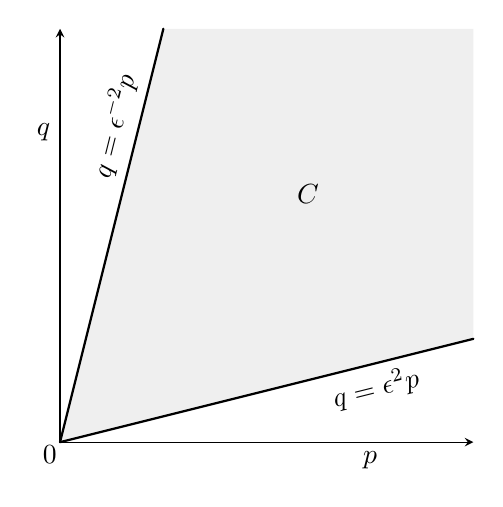
\begin{tikzpicture}[x=5.25cm, y=5.25cm, line cap=round, >=stealth]

%% Dessin du cône.

\fill[gray!12.5] (0,0) -- (.25,1) -- (1,1) -- (1,.25) -- cycle ;
\draw[thick] (0,0) -- node[near end,sloped,above]{$q=\epsilon^{-2}p$} (.25,1) ;
\draw[thick] (0,0) -- node[near end,sloped,below]{$q=\epsilon^2  p$} (1,.25) ;

%% Le carré contenant le cône.

\node[anchor=north east, inner sep=1pt] (0,0) {$0$};
\draw[thin,->] (0,0) -- node[near end,anchor=north]{$p$} (1,0);
\draw[thin,->] (0,0) -- node[near end,anchor=east ]{$q$} (0,1);

%% Nom des zones.

\node at (.6,.6) {$C$};

\end{tikzpicture}
%
\hfill
%
\begin{tikzpicture}[x=5.25cm, y=5.25cm, line cap=round, >=stealth]

%% Dessin du cône.

%% Le carré contenant le cône.

\node[anchor=north east, inner sep=1pt] (0,0) {$0$};
\draw[thin,->] (0,0) -- node[near end,anchor=north]{$p$} (1,0);
\draw[thin,->] (0,0) -- node[near end,anchor=east ]{$q$} (0,1);

%% Nuage de points.

\begin{scope}[ultra thin]
\input{mustar-data-2048}
\end{scope}

\end{tikzpicture}
%
\caption{The measure~$\mu^*$. On the left, the different zones for the measure;
on the right, a Poisson cloud of points with density $\mu^*$.
The scale and density of the cloud are consistent with Figure~\ref{fig-mu}.}%
\label{fig-mustar}
%
\end{figure}
%
So, near $0$, $\mathcal{L}$ behaves like the operator $\mathcal{L}^*$ on~$L^2(0,\infty)$
defined by:
\[\label{fo4259}
\big(\mathcal{L}^*f\big)(p) = \int_{\epsilon^2p}^{\epsilon^{-2}p} \frac{\epsilon}{4\sqrt{pq}} \dx{q}
+ \frac{\epsilon^2}{2} f(\epsilon^2p) + \frac{1}{2} f(\epsilon^{-2}p) .\]

$\mathcal{L}^*$ has scale invariance properties which make it easy to study.
One finds that $\mathcal{L}^*$ is self-adjoint,
that its spectral radius is $\Lambda$,
and that it has $\Lambda$ as a quasi-eigenvalue, associated with the quasi-eigenvector
$(p\mapsto1/\sqrt{p})$.
So, you see that it suffices to study the `local' operator $\mathcal{L}^*$
to compute the spectral radius of the `global' operator $\mathcal{L}$;
in other words, there is a phenomenon of `localization of the spectral radius'
for~$\mathcal{L}$.
\end{Rmk}


\subsection{Optimality of the strong event sufficient condition}%
\label{parOptimalityOfTheStrongEventSufficientCondition}

Now I will prove that Theorem~\ref{thm0367b} is optimal:
%
\begin{Thm}\label{pro1616}
The factor $\Lambda(\epsilon)$ in~(\ref{for7753}) cannot be improved.
In other words, for all~$\Lambda'<\Lambda(\epsilon)$ it is possible to find
$\sigma$-fields~$\mathcal{F}$ and~$\mathcal{G}$ satisfying
\[\label{for8717}
\forall A \in \mathcal{F}, B \in \mathcal{G} \quad \Pr[A\cap B] - \Pr[A]\Pr[B] \leq \epsilon \sqrt{\Pr[A]\Pr[\C{A}]\Pr[B]\Pr[\C{B}]}, \]
but such that $\{\mathcal{F}:\mathcal{G}\} \geq \Lambda'$.
\end{Thm}
%
\begin{Rmk}
One can automatically add absolutes values
in the left-hand side of the condition~(\ref{for8717}),
since $-\big(\Pr[A\cap B] - \Pr[A]\Pr[B]\big) = \Pr[A\cap \C{B}] - \Pr[A]\Pr[\C{B}]$.
\end{Rmk}

Actually I will rather prove the following statement,
which is equivalent to the theorem by continuity of the function~$\Lambda(\Bcdot)$:
\begin{Clm}
For all~$\epsilon'>\epsilon$ it is possible to find $\sigma$-fields~$\mathcal{F}$ and~$\mathcal{G}$
satisfying $\{\mathcal{F}:\mathcal{G}\} \geq \Lambda(\epsilon)$, but such that
\[\label{for8717b}
\forall A \in \mathcal{F}, B \in \mathcal{G} \quad \Pr[A\cap B] - \Pr[A]\Pr[B] \leq \epsilon' \sqrt{\Pr[A]\Pr[\C{A}]\Pr[B]\Pr[\C{B}]} .\]
\end{Clm}

\begin{proof}
According to the proof of Theorem~\ref{thm0367b},
the `natural' proof would be to take for space $(\Omega,\mathcal{B},\Pr)$
the set $(0,1)^2$ equipped with its Borel $\sigma$-field
and endowed with the Chogosov law~$\mu$,
and to set $\mathcal{F} = \sigma(p)$ and $\mathcal{G} = \sigma(q)$.
%
Though it seems to be true that that system satisfies~(\ref{for0256b}),
the complicated structure of~$\mu$ makes existence of a short proof for that property unlikely.
Therefore I will rather adapt the previous idea
to the nicer measure~$\mu^*$ defined by~(\ref{fo4208}),
or more precisely to a `truncation' of it.

My system is the following:
$(\Omega,\mathcal{B},\Pr)$ is the set $(0,1)^2$
equipped with its Borel $\sigma$-field and endowed with a certain measure~$\nu$
(specified just after), and I take $\mathcal{F} = \sigma(p)$, resp.\ $\mathcal{G} = \sigma(q)$.
The measure~$\nu$, which depends on some parameter $x \in (0,1)$ morally close to~$0$,
is a measure on~$(0,1)^2$ having uniform marginals,
which coincides with~$\mu^*$ on~$(0,x]^2$
and which is `as uniform as possible' outside $(0,x]^2$ (see Figure~\ref{fig-nu}).
Technically:
%
\[ \nu[A\times B] = \begin{cases}
\mu^*(A\times B) & \text{if $A \subset (0,x]$ and $B \subset (0,x]$;} \\
0 & \text{if $A \subset (0,\epsilon^2x]$ and $B \subset (x,1)$;} \\
0 & \text{if $A \subset (x,1)$ and $B \subset (0,\epsilon^2x]$;} \\
\big[ \int_A \big( 1 - \frac{\epsilon}{2}\sqrt{\frac{x}{p}} \big) \dx{p} \big] |B| \big/ (1-x)
& \text{if $A \subset (\epsilon^2x,x]$ and $B \subset (x,1)$;} \\
|A| \big[ \int_B \big( 1 - \frac{\epsilon}{2}\sqrt{\frac{x}{q}} \big) \dx{q} \big] \big/ (1-x)
& \text{if $A \subset (x,1)$ and $B \subset (\epsilon^2x,x]$;} \\
{[}1-(2-\epsilon)x] |A| |B| / (1-x)^2 & \text{if $A \subset (x,1)$ and $B \subset (x,1)$.}
\end{cases} \]
%
\begin{figure}
\centering
%
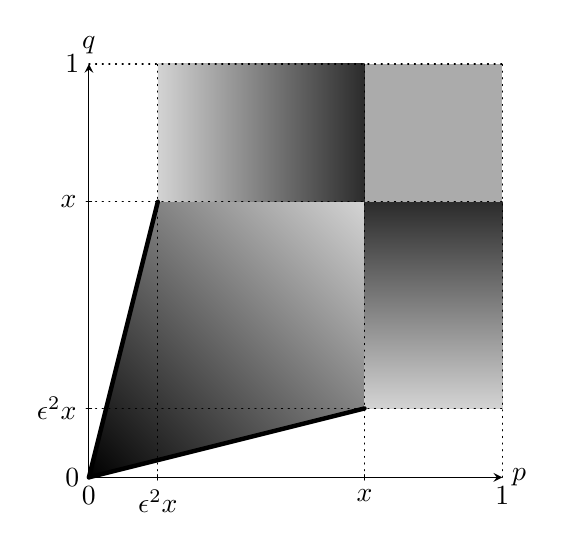
\begin{tikzpicture}[x=5.25cm, y=5.25cm, line cap=round, >=stealth]

\begin{scope}
\clip[draw] (0,0) -- (.1667,.6667) -- (.6667,.6667) -- (.6667,.1667) -- cycle ;
\shade[top color=black!100,bottom color=black!17,shading angle=135] (.3333,.3333) circle (.4714);
\end{scope}

\shade[left color=black!17,right color=black!83] (.1667,.6667) rectangle (.6667,1) ;
\shade[bottom color=black!17,top color=black!83] (.6667,.1667) rectangle (1,.6667) ;
\fill[black!33] (.6667,.6667) rectangle (1,1) ;

\draw[ultra thick] (0,0) -- (.1667,.6667) ;
\draw[ultra thick] (0,0) -- (.6667,.1667) ;
\draw[thin,dotted] (.1667,0) -- +(0,1) ;
\draw[thin,dotted] (.6667,0) -- +(0,1) ;
\draw[thin,dotted] (1,0) -- +(0,1) ;
\draw[thin,dotted] (0,.1667) -- +(1,0) ;
\draw[thin,dotted] (0,.6667) -- +(1,0) ;
\draw[thin,dotted] (0,1) -- +(1,0) ;

\draw[->,thin] (0,0) node[anchor=north]{$0$} --
(1,0) node[anchor=north]{$1$} node[anchor=west]{$p$} ;
\draw[->,thin] (0,0) node[anchor=east]{$0$} --
(0,1) node[anchor=east]{$1$} node[anchor=south]{$q$} ;

\draw (.1667,0) +(0,1pt) -- +(0,-1pt) node[anchor=north]{$\epsilon^2x$} ;
\draw (.6667,0) +(0,1pt) -- +(0,-1pt) node[anchor=north]{$x$} ;
\draw (0,.1667) +(1pt,0) -- +(-1pt,0) node[anchor=east ]{$\epsilon^2x$} ;
\draw (0,.6667) +(1pt,0) -- +(-1pt,0) node[anchor=east ]{$x$} ;

\end{tikzpicture}
%
\caption{A schematic representation of the measure~$\nu$.}%
\label{fig-nu}
\end{figure}

\noindent\textit{First step: Proof that $\{\mathcal{F}:\mathcal{G}\} \geq \Lambda$.}\quad
Let~$\Lambda' < \Lambda$.
Since $\Lambda$ is in the spectrum of the self-adjoint operator $\mathcal{L}^*$ on~$L^2(0,\infty)$
(see~(\ref{fo4259}) and the lines just below),
there exists $f \in L^2(0,\infty)\setminus\{0\}$
such that $\langle \mathcal{L}^*f,f \rangle / \|f\|_{L^2(0,\infty)} > \Lambda'$.
By a standard truncation argument, we can assume that $f$ has bounded support,
say that $f$ is zero outside $(0,Y]$.
Dividing $f$ by its norm we can also assume that $\|f\|_{L^2} = 1$.

Now, for~$y \in (0,x]$ define the function~$f_y$ by:
\[ f_y(p) \coloneqq \sqrt{\frac{Y}{y}} \, f \! \bigg(\frac{Y}{y}p\bigg) .\]
$f_y$ is zero outside $(0,y] \allowbreak {\subset (0,x]}$; it satisfies $\|f_y\|_{L^2} = 1$ and
\[ \langle \mathcal{L}^*f_y, f_y \rangle = \langle \mathcal{L}^*f,f \rangle > \Lambda' \]
by the scale invariance properties of~$\mathcal{L}^*$.

Denote $m \coloneqq \int f(p) \,\dx{p} / \sqrt{Y}$, which is finite since $f$ is $L^2$ with compact support;
one has $\int f_y(p) \,\dx{p} = \sqrt{y}m$,
so the projection of~$f_y$ on~$\ldb(0,1)$ is the function~$\bar{f}_y = f_y-\sqrt{y}m$.
One has $\|\bar{f}_y\|_{\ldb(0,1)} \leq \|f_y\|_{L^2} = 1$,
and
\[ \EE\big[ \bar{f}_y(p)\bar{f}_y(q) \big] = \langle \mathcal{L}^*f_y,f_y \rangle - m^2y
> \Lambda' - m^2y ,\]
so that $\{\mathcal{F}:\mathcal{G}\} > \Lambda' - m^2y$. Making $y \longto 0$
and then $\Lambda' \longto \Lambda$, one finally gets $\{\mathcal{F}:\mathcal{G}\} \geq \Lambda$.

\noindent\textit{Second step: Proof of~(\ref{for8717b}).}\quad
Let~$\epsilon'>\epsilon$; we want to prove that, provided $x$ is small enough,
(\ref{for8717b}) is satisfied.

Let~$A$ and~$B$ be resp.\ $\mathcal{F}$- and $\mathcal{G}$-measurable events.
One can assume safely that $|A| \leq 1/2$,
since replacing simultaneously~$A$ by~$\C{A}$ and~$B$ by~$\C{B}$ leaves
both sides of~(\ref{for8717b}) unchanged.
%
One can also assume that $|B| < 1/(1+\epsilon^2)$,
since for $|B|\geq1/(1+\epsilon^2)$, (\ref{for8717b}) comes `for nothing'
by writing
\[ \Pr[A\cap B] - \Pr[A]\Pr[B] \leq \Pr[A](1-\Pr[B]) \leq
\sqrt{\Pr[A]\Pr[\C{A}]} \times \epsilon \sqrt{\Pr[B]\Pr[\C{B}]}
.\]

\begin{NOTA}
In the sequel of this proof we indentify~$A$ and~$B$ with Borel subsets of~$(0,1)$,
rewriting the $p$-measurable event $A$ into the set $A\times(0,1)$, resp.\
the $q$-measurable event $B$ into the set $(0,1)\times B$.
Since both marginals of~$\nu$ are uniform on~$(0,1)$,
one then has $\Pr[A]=|A|$, resp.\ $\Pr[B]=|B|$, so that our goal becomes proving:
\[ \nu[A\times B] - |A||B| \leq \epsilon' \sqrt{|A||B||\C{A}||\C{B}|} .\]
\end{NOTA}

Denote $\check{A} \coloneqq A\cap(0,x]$, resp.\ $\check{B} \coloneqq B\cap(0,x]$.
Provided $x\leq\epsilon/2$, the signed measure~$\dx\nu(p,q) - \dx{p}\dx{q}$ is nonpositive
on~$(0,x]\times(x,1) \cup (x,1)\times(0,x]$,
so that
\[\label{for1899}
\nu[A\times B] - |A||B| \leq
\nu\big[\check{A}\times\check{B}\big] - |\check{A}| |\check{B}|
+ \nu\big[(A\setminus\check{A})\times(B\setminus\check{B})\big]
- \big|A\setminus\check{A}\big| \big|B\setminus\check{B}\big| .\]

Now let us bound above the right-hand side of~(\ref{for1899}):
\begin{itemize}
\item The second term is obviously nonpositive.
%
\item The third term is $[1-(2-\epsilon)x] \* |A\setminus\check{A}| \* |B\setminus\check{B}| \div (1-x)^2$, so the sum of the two last terms is~%
${(\epsilon x-x^2)} \* {|A\setminus\check{A}|} \* {|B\setminus\check{B}|} \div
(1-x)^2 \ab \leq (\epsilon x - x^2) \* |A| |B|/ \* (1-x)^2$.
Since $|A| \leq 1/2$ and $|B| \leq 1/\allowbreak{(1+\epsilon^2)}$, that quantity
is in turn bounded by~$\frac{\epsilon x-x^2}{\epsilon(1-x)^2} \times
\sqrt{|A||B||\C{A}||\C{B}|}$.
%
\item For the first term, by Lemma~\ref{clm8768} stated just below, one has
$\nu\big[\check{A}\times \check{B}\big] = \mu^*\big[\check{A}\times \check{B}\big]
\leq \epsilon \sqrt{\mathsmaller{\big|\check{A}\big|\big|\check{B}\big|}}
\leq \epsilon \sqrt{\mathsmaller{\big|\check{A}\big|\big|\C{\check{A}}\big|\big|\check{B}\big|\big|\C{\check{B}}\big|}} \div (1-x)$,
%
in which, provided $x \leq \epsilon^2 \div (1+\epsilon^2)$, one has
$\sqrt{\mathsmaller{\big|\check{B}\big|\big|\C{\check{B}}\big|}} \leq \sqrt{B|\C{B}|}$
(because then $|\check{B}| \leq |B|\wedge x$ and $|B| \leq 1-x$),
and similarly $\sqrt{\mathsmaller{\big|\check{A}\big|\big|\C{\check{A}}\big|}} \leq \sqrt{A|\C{A}|}$,
so that in the end the first term is bounded by
$\frac{\epsilon}{1-x} \sqrt{|A||B||\C{A}||\C{B}|}$.
\end{itemize}
%
Summing things up, we get:
\[\label{f4004} \nu[A\times B] - |A||B| \leq
\bigg( \frac{\epsilon}{1-x} + \frac{\epsilon x-x^2}{\epsilon(1-x)^2} \bigg)
\sqrt{|A||B||\C{A}||\C{B}|} .\]
Taking $x$ sufficiently close to~$0$,
the first factor of the right-hand side of~(\ref{f4004}) is $\leq\epsilon'$,
whence the second step of the proof.
\end{proof}

\begin{Lem}\label{clm8768}
For all~$A,B \subset (0,\infty)^2$ with Lebesgue measures $|A|,|B| \ab {<\infty}$,
${\mu^*[A\times B]} \leq \epsilon \sqrt{|A||B|}$.
\end{Lem}
%
\begingroup\def\proofname{Proof of Lemma~\ref{clm8768}}
\begin{proof}
Recall that $\mu^*$ is the Radon measure on~$(0,\infty)^2$
having density $\epsilon/4\sqrt{pq}$ w.r.t.\ the Lebesgue measure
inside the cone $C = \{(p,q)\colon \epsilon^2p<q<\epsilon^{-2}p\}$,
being zero outside~$C$,
and giving to the borders of~$C$ a lineic mass defined by
$\mu^*\{ (p,\epsilon^2p) \colon p \in A \} = \epsilon^2|A|/2$, resp.\ 
$\mu^*\{ (p,\epsilon^{-2}p) \colon p \in A \} = |A|/2$ (see Figure~\ref{fig-mustar}).
$\mu^*$ is invariant under switching~$p$ and~$q$,
and its marginals both are the Lebesgue measure on~$(0,\infty)$.
Let~$A, B \subset (0,\infty)$ be Borel;
our goal is to show that $\mu^*[A\times B] \leq \epsilon\sqrt{|A||B|}$.

\newcounter{step}
\newcommand{\step}{\addtocounter{step}{1}\textbf{\textit{Step \arabic{step}}.}\quad}
\step If $|A| \leq \epsilon^2|B|$ the result is trivially true,
since then $\mu^*[A\times B] \leq \mu^*[A\times (0,\infty)] = |A| \leq \epsilon\sqrt{|A||B|}$.
Similarly the result is true if $|B| \leq \epsilon^2|A|$.
Therefore in our proof we will always assume that $\epsilon^2|A| < |B| < \epsilon^{-2}|A|$.

\step As for the measure~$\mu$,
decompose the support of~$\mu^*$ into three parts~%
$\mfrak{U}$, \twocirc\ and~$\mfrak{D}$, corresponding resp.\
to the line ``$p=\epsilon^2q$'', the cone $C$ and the line ``$p=\epsilon^{-2}q$''
(see Figure~\ref{fig-mustar}).
Write $\mu^*[A\times B] = m_U + m_2 + m_D$,
where $m_U = \mu^*[(A\times B)\cap\mfrak{U}]$, etc..

Denote by~$\mu^*_q$ the `conditioned version' of~$\mu$ knowing~$q$, i.e. the probability measure such that
\[ \mu^*[X] = \int_0^{\infty} \mu^*_q [\{p\colon (p,q)\in X\}] \,\dx{q} ,\]
which can be computed explicitly to be:
\[\label{for7553} \dx\mu^*_q[p] = \1{\{p=\epsilon^2q\}} \frac{\epsilon^2}{2}
+ \1{\{\epsilon^2q<p<\epsilon^{-2}q\}} \frac{\epsilon}{4\sqrt{pq}} \dx{p} + \1{\{p=\epsilon^{-2}q\}} \frac{1}{2} .\]
%
The three terms of the right-hand side of~(\ref{for7553}) are respectively due
to~$\mfrak{U}$, $\twocirc$ and~$\mfrak{D}$, so that, integrating the first one, one finds:
\[ m_U = \int_B \frac{\epsilon^2}{2} \1{\{A\ni\epsilon^2q\}} \dx{q}
\leq \frac{\epsilon^2}{2} |B| .\]
Switching the roles of~$p$ and~$q$,
one has similarly $m_D \leq \epsilon^2|A|/2$.
Then it only remains to bound~$m_2$.

\step Let us study further the measures $\mu^*_q$.
If $q\in\epsilon^2A$, then $A\ni\epsilon^{-2}q$
and thus $\mu^*_q[A] \geq \mu^*[\{\epsilon^{-2}q\}] = 1/2$,
and conversely if $q\notin\epsilon^2A$, then $A\not\ni\epsilon^{-2}q$
and thus $\mu^*_q[A] \leq 1-\mu^*[\{\epsilon^{-2}q\}] = 1/2$.
So, $\mu^*_q[A]$ is never smaller if $q\in\epsilon^2A$
than if $q\notin\epsilon^2A$.

As a consequence, let us show that we can always assume
that $\epsilon^2A \subset B$.
Since $|B|>\epsilon^2|A|$,
$|B\setminus \epsilon^2A| > |\epsilon^2A\setminus B|$,
so we can fix some $B^- \subset B\setminus \epsilon^2A$
such that $|B^-| = |\epsilon^2A\setminus B|$.
One has:
\[\label{c7947}
\mu^*[A\times B^-] = \int_{B^-} \mu^*_q(A) \,\dx{q} \leq \frac{|B^-|}{2} \\
= \frac{|\epsilon^2A\setminus B|}{2}
\leq \int_{\epsilon^2A\setminus B} \mu^*_q(A) \,\dx{q}
= \mu^*[A\times(\epsilon^2A\setminus B)] .
\]
%
Shorthanding ``$(B\setminus B^-)\cup\epsilon^2A$'' into ``$B'$'', (\ref{c7947}) implies that
replacing $B$ by~$B'$ —which does not modify the value of~$|B|$ —%
cannot make $\mu^*[A\times B]$ decrease.
Consequently, if we prove that ${\mu^*[A\times B']} \leq \epsilon\sqrt{|A||B'|}$,
then we will also have proved that $\mu^*[A\times B] \leq \epsilon\sqrt{|A||B|}$.
As $\epsilon^2A\subset B'$, we thus have demonstrated the statement
at the beginning of this paragraph:
one can always assume that $\epsilon^2A\subset B$.

\begin{NOTA}
Switching the roles of~$p$ and~$q$, we will rather impose,
instead of~$\epsilon^2A\subset B$, that $\epsilon^2B\subset A$.
\end{NOTA}

\step Call~$\mu^{\circ}$ the measure~$\mu^*$ restricted to~$C$,
i.e.\ $\dx\mu^{\circ} = \1{C}\dx\mu^*$,
so that $m_2 = \mu^{\circ}[A\times B]$.
$\mu^{\circ}$ is absolutely continuous w.r.t.\ the Lebesgue measure;
denote by~$\mu^{\circ}_q$ its `conditioned version' for fixed~$q$,
i.e.\ the measure such that
\[ \mu^{\circ}[X] = \int_0^\infty \mu^{\circ}_q \big[\big\{p\colon (p,q)\in X\big\}\big] \,\dx{q} ,\]
which has the following explicit density w.r.t.\ the Lebesgue measure:
\[ \label{for5093} \dx\mu^{\circ}_q[p] =
\1{\{\epsilon^2q<p<\epsilon^{-2}q\}} \frac{\epsilon}{4\sqrt{pq}} \,\dx{p} .\]
%
We perform a change of variables:
for~$y\in(0,|B|)$, define
\[ \beta(y) = \inf\big\{ q\in(0,\infty) \colon |B\cap(0,q)| \geq y \big\} ;\]
so that the push-forward $\beta\pushfwd\dx{q}$
of the Lebesgue measure on~$(0,|B|)$ by the map $\beta$
is equal to~$\1{B}\dx{q}$, the Lebesgue measure restricted to~$B$;
then
\[ m_\text{\twocirc} = \int_B \mu^{\circ}_q[A] \,\dx{q} =
\int_0^{|B|} \mu^{\circ}_{\beta(y)}[A] \,\dx{y} .\]
Our strategy will consist in bounding $\mu^{\circ}_{\beta(y)}[A]$ for all~$y$.

First, we observe that there is some portion of~$A$ which does not contribute to~$\mu^\circ_{\beta(y)}[A]$.
Denote indeed $A_y \coloneqq \{ \epsilon^2q \colon q\in B\cap(0,\beta(y)) \}$;
by the definition of~$\beta$, $|A_y| = \epsilon^2y$,
and one has $A_y \subset \epsilon^2B \subset A$.
But $A_y \subset (0,\epsilon^2\beta(y))$,
so $\mu^{\circ}_{\beta(y)}[A_y] = 0$,
and thus $\mu^{\circ}_{\beta(y)}[A] = \mu^{\circ}_{\beta(y)}[A\setminus A_y]$,
where $|A\setminus A_y| = |A| - |A_y| = |A| - \epsilon^2y$.

Now, for~$q\in(0,\infty)$, the density of~$\mu^{\circ}_q$ is zero for $p\leq\epsilon^2q$
and it is nonincreasing for $p>\epsilon^2q$,
so an immediate coupling argument shows that the maximal value of
$\mu^{\circ}_q[X]$ under the constraint ``$|X|=x$'' is attained for
$X = (\epsilon^2q,\epsilon^2q+x)$.
Applying that result to the conclusion of the previous paragraph, we get that:
%
\[\label{f1291} \mu^{\circ}_{\beta(y)}[A] \leq
\mu^{\circ}_{\beta(y)} \big[\big(\epsilon^2\beta(y)\,,\,\epsilon^2\beta(y)+|A|-\epsilon^2y\big)\big] .\]
%
But for~$x\geq 0$, the quantity
$ \mu^{\circ}_q[(\epsilon^2q\,,\,\epsilon^2q+x)] $
can be computed explicitly to be
\[ \mu^{\circ}_q \big[\big(\epsilon^2q\,,\,\epsilon^2q+x\big)\big] =
\left\{\begin{array}{lcl} (1-\epsilon^2)/2 & \quad & \text{if $q\leq x/(\epsilon^{-2}-\epsilon^2)$;} \\
\big( \epsilon \sqrt{\epsilon^2+x/q} - \epsilon^2 \big) /2 & \quad & \text{if $q>x/(\epsilon^{-2}-\epsilon^2)$.} \end{array}\right.\]
In particular, that quantity is a nonincreasing function of~$q$.
Since, by the definition of~$\beta$, one always has $\beta(y) \geq y$,
it follows that (\ref{f1291}) can be improved into:
%
\[ \mu^\circ_{\beta(y)}[A] \leq \mu^\circ_y [(\epsilon^2y\,,\,|A|)] =
\left\{\begin{array}{lcl} (1-\epsilon^2)/2 &\quad& \text{if $y\leq\epsilon^2|A|$;} \\
\big( \epsilon\sqrt{|A|/y} - \epsilon^2 \big) /2 &\quad& \text{if $y>\epsilon^2|A|$.} \end{array}\right.\]
%
Integrating, one finds finally:
\begin{multline}
m_2 \leq \int_0^{\epsilon^2|A|} \frac{1-\epsilon^2}{2} \dx{y} + \int_{\epsilon^2|A|}^{|B|}
\bigg( \frac{\epsilon\sqrt{|A|}}{2\sqrt{y}} - \frac{\epsilon^2}{2} \bigg) \dx{y} \\
= \frac{(1-\epsilon^2)\epsilon^2|A|}{2} + \bigg[ \epsilon\sqrt{|A|y} - \frac{\epsilon^2y}{2} \bigg]^{|B|}_{\epsilon^2|A|}
= \epsilon\sqrt{|A||B|} - \frac{\epsilon^2}{2} \big(|A|+|B|\big).
\end{multline}

\step We put our bounds together to get the lemma:
\[ \mu^*[A\times B] \leq m_D + m_U + m_2
= \frac{\epsilon^2}{2} \big(|A|+|B|\big) + \epsilon\sqrt{|A||B|} - \frac{\epsilon^2}{2} \big(|A|+|B|\big)
= \epsilon\sqrt{|A||B|} .\]
\end{proof}\endgroup

\begin{Rmk}
A careful reading of the proof above shows
that the maximal value of~$\mu^*[A\times B]$ is attained for
$A = (0,|A|), B=(0,|B|)$, in which case, provided $\epsilon^2|A|\leq|B|\leq\epsilon^{-2}|A|$,
one has equality in Lemma~\ref{clm8768}.
\end{Rmk}

